% Bio Inspired Algorithms AAT report: Bio-inspired feature selection for medical image classification.
% Layout follows the department LaTeX report template (page border, chapter style, headers and footers).
% Every result comes from the project outputs (Derma/README.md, docs/project_writeup.md) and matches the deck.
% Overleaf: upload this file, logo.png (department logo) and figures/test_scores.png, then compile with pdfLaTeX.
\documentclass[12pt,a4paper]{report}
\usepackage{lmodern}
\usepackage{graphicx}
\usepackage{amsmath}
\usepackage{amssymb}
\usepackage{url}
\usepackage{hyperref}
\usepackage{setspace}
\usepackage{geometry}
\usepackage{background}
\usepackage{titlesec}
\usepackage{tabularx}
\usetikzlibrary{calc,arrows.meta,positioning}
\usepackage{etoolbox}
\usepackage{float}
\usepackage{multirow}
\usepackage{algorithm}
\usepackage{algorithmic}
\usepackage{xcolor}

\definecolor{violet}{HTML}{5237E6}
\definecolor{lavender}{HTML}{B8A7FF}
\definecolor{ink}{HTML}{3D3D3D}

% Links in blue, as in the department template
\hypersetup{
    colorlinks=true,
    citecolor=blue,
    linkcolor=blue,
    urlcolor=blue
}

\renewcommand{\algorithmicrequire}{\textbf{Input:}}
\renewcommand{\algorithmicensure}{\textbf{Output:}}

\geometry{
 a4paper,
 total={170mm,257mm},
 left=20mm,
 top=20mm,
}

% Page border on every page
\backgroundsetup{angle=0, scale=1, vshift=-5ex,
  contents={\tikz[overlay, remember picture]
    \draw [rounded corners=7pt, line width=1.8pt,
           color=black, fill=white!50, double=black!120]
           ($(current page.north west)+(0.4cm,-0.4cm)$)
           rectangle ($(current page.south east)+(-0.4,0.4)$);}}

\titleformat{\chapter}[display]
  {\normalfont\bfseries}
  {\makebox[\textwidth][l]{\fontsize{36}{42}\selectfont\chaptername\ \thechapter}}
  {0pt}
  {\centering\fontsize{28}{34}\selectfont}
  []
\titlespacing*{\chapter}{0pt}{0pt}{14pt}

\titleformat{\section}
  {\normalfont\fontsize{12}{14}\bfseries}{\thesection}{1em}{}
\titlespacing*{\section}{0pt}{*2}{*1.5}

\titleformat{\subsection}
  {\normalfont\fontsize{12}{14}\bfseries\itshape}{\thesubsection}{1em}{}
\titlespacing*{\subsection}{0pt}{*1.5}{*1}

\titleformat{\subsubsection}
  {\normalfont\fontsize{12}{14}\bfseries\itshape}{\thesubsubsection}{1em}{}
\titlespacing*{\subsubsection}{0pt}{*1}{*0.5}

\usepackage{fancyhdr}
\fancypagestyle{plain}{%
  \fancyhf{}
  \renewcommand{\headrulewidth}{0pt}
  \renewcommand{\footrulewidth}{0pt}
}
\fancypagestyle{chapterstyle}{%
  \fancyhf{}
  \fancyhead[L]{\leftmark}
  \fancyhead[R]{\thepage}
  \fancyfoot[C]{\small B.M.S College of Engineering, Bangalore}
  \renewcommand{\headrulewidth}{1.5pt}
  \renewcommand{\footrulewidth}{1.0pt}
}

\renewcommand{\bibname}{References}
\newcommand{\projecttitle}{Bio-Inspired Feature Selection for Medical Image Classification: Genetic Algorithm and Competitive Swarm Optimisation on MedMNIST}
% The department logo; the document still compiles if logo.png has not been uploaded yet.
\newcommand{\logo}[2]{\IfFileExists{logo.png}{
\includegraphics[#1]{logo.png}\\[#2]}{}}

\begin{document}
\linespread{1.39}\selectfont
\pagestyle{plain}

% ============================================================ COVER
\begin{titlepage}
    \begin{center}
        \textsc{\Large \textbf{\textcolor{blue}{B.M.S. COLLEGE OF ENGINEERING}}}\\[0.2cm]
        \textsc{\large \textbf{(Autonomous College under VTU)}}\\[0.2cm]
        \textsc{\large \textbf{Bull Temple Road, Basavangudi, Bangalore - 560019}}\\[0.5cm]

        \logo{scale=0.75}{0.2cm}
        \textit{A Bio Inspired Algorithms AAT report on}\\[0.2cm]
        \textsc{\textbf{\textcolor{red}{\projecttitle}}}\\[0.2cm]
        \textit{in fulfillment of the requirements for the award of degree}\\[0.2cm]

        \textbf{BACHELOR OF ENGINEERING}\\[0.15cm]
        \textit{in}\\[0.2cm]
        \textbf{Computer Science \& Engineering (Data Science)}\\[0.2cm]

        \textit{by}\\[0.2cm]
        \textbf{Alvin S Thottappilly (1BM23CD005)}\\[0.2cm]
        \textbf{Chinmayee S Bharadwaj (1BM23CD012)}\\[0.2cm]
        \textbf{Taran Thimmaiah (1BM23CD065)}\\[0.85cm]

        \textbf{Under the Guidance of}\\[0.25cm]
        \textbf{Manoj Kumar}\\[0.15cm]
        Assistant Professor\\[0.55cm]
        \textbf{Department of CSE (Data Science)}, \\
        \textbf{B.M.S. College of Engineering}\\[0.3cm]

        \textbf{AY 2026-2027}
    \end{center}
\end{titlepage}

% ============================================================ CERTIFICATE
% Tighter line spacing on this page only, so the examiner lines stay on it with the logo in place.
\begingroup
\linespread{1.15}\selectfont
\begin{center}
    \textsc{\Large \textbf{\textcolor{blue}{B.M.S. COLLEGE OF ENGINEERING}}}\\[0.1cm]
    \textsc{\large \textbf{(Autonomous College under VTU)}}\\[0.1cm]
    \textsc{\large \textbf{Bull Temple Road, Basavangudi, Bangalore - 560019}}\\[0.25cm]

    \logo{scale=0.35}{0.1cm}
    \textbf{Department of Computer Science and Engineering}\\
    \textbf{(Data Science)}\\[0.1cm]
    \textbf{\Large \underline{CERTIFICATE}}\\[0.1cm]
\end{center}

\noindent
This is to certify that the project entitled ``\textbf{\projecttitle}'' is a bona fide work carried out by the
following students for the course Bio Inspired Algorithms (Course Code: \textbf{23DS7BSBIO}). It is certified that
all corrections and suggestions indicated during the internal assessments have been incorporated in the final report
submitted to the departmental library. The project report has been approved as it meets the academic requirements
prescribed for the Bachelor of Engineering Degree in respect of project work.

\begin{center}
    \textbf{\underline{Candidate details}}\\[0.2cm]
\begin{tabularx}{\textwidth}{|c|X|c|c|}
    \hline
    \textbf{SL. NO.} & \textbf{Student Name} & \textbf{USN} & \textbf{Student's Signature} \\
    \hline
    1 & Alvin S Thottappilly & 1BM23CD005 & \\
    \hline
    2 & Chinmayee S Bharadwaj & 1BM23CD012 & \\
    \hline
    3 & Taran Thimmaiah & 1BM23CD065 & \\
    \hline
\end{tabularx}
\end{center}

\vspace{0.2cm}

\noindent
\textbf{Signature of the Guide}\hfill \textbf{Signature of the HOD}\\[0.4cm]
\textbf{Manoj Kumar}\hfill \textbf{Dr. Shyamala G}\\
Assistant Professor \hfill Professor \& HOD\\[0.1cm]

\begin{center}
    \textbf{Examiners}
\end{center}
\vspace{-0.4cm}
\noindent
    \textbf{Name of Examiner} \hfill \textbf{Signature of the examiner} \\[0.25cm]
    \textbf{1.} \hfill \rule{5cm}{0.4pt} \\[0.25cm]
    \textbf{2.} \hfill \rule{5cm}{0.4pt}
\endgroup

\newpage

% ============================================================ ACKNOWLEDGEMENTS
\chapter*{\centering Acknowledgements}
\addcontentsline{toc}{chapter}{Acknowledgements}

We would like to take this opportunity to express our heartfelt gratitude to \textbf{Dr.\ B.\ S.\ Ragini Narayan},
Chairperson, Donor Trustee, Member Secretary \& Chairperson, BMSET; \textbf{Dr.\ P.\ Dayananda Pai}, Member Life
Trustee, BMSET; and \textbf{Dr.\ Bheemsha Arya}, Principal, B.M.S. College of Engineering, for providing the
infrastructure needed to complete this Alternative Assessment.

We wish to express our deepest gratitude and thanks to \textbf{Dr.\ Shyamala G}, Head of the Department,
Computer Science and Engineering (Data Science), and to our project guide \textbf{Manoj Kumar}, Assistant
Professor, for their constant support, guidance and encouragement throughout this work.

A warm thanks to all the faculty of the Department of Computer Science and Engineering (Data Science), who helped
us with their views and encouraging ideas. We also thank the creators of the MedMNIST benchmark and the open-source
libraries used in this project.

\newpage
\tableofcontents

\begin{center}
    \listoftables
\end{center}

\begin{center}
    \listoffigures
\end{center}

\newpage

% ============================================================ ABSTRACT
\chapter*{\centering Abstract}
\addcontentsline{toc}{chapter}{Abstract}

Bio-inspired metaheuristics such as the Genetic Algorithm (GA) and Particle Swarm Optimisation (PSO) are widely
used to select subsets of image features for medical image classification. This project asks when such algorithms
actually improve a classifier, and tests the question under strict, fair conditions on four datasets from the
MedMNIST benchmark: breast ultrasound, retinal fundus, chest X-ray and dermatoscopy images.

Every comparison used equal evaluation budgets, a random-search control with the same budget, paired random seeds,
a test set scored only once, and Wilcoxon signed-rank tests with Holm correction for multiple comparisons. On
features taken from trained ResNet-18 networks, eight nature-inspired algorithms (GA, PSO, binary PSO with S- and
V-shaped transfer functions, Grey Wolf Optimiser, Whale Optimisation Algorithm, Harris Hawks Optimisation and the
Competitive Swarm Optimiser) gave no significant improvement in six controlled studies, because the deep features
are highly redundant.

On 1,820 handcrafted radiomics features (texture, shape, colour and frequency descriptors) extracted from 10,015
DermaMNIST skin-lesion images, with a fixed budget of 50 features, GA and the Competitive Swarm Optimiser (CSO)
selected significantly better features than both random search and a standard ANOVA filter. With a support vector
machine, GA reached a test accuracy of 78.3\% against 77.0\% for random search and 76.5\% for the filter (gains of
1.38 and 1.88 percentage points) and a test AUC of 0.936 against 0.925 and 0.928. All 16 pre-specified comparisons,
with both an SVM and a k-nearest-neighbour classifier, were statistically significant. The selected models use only
2.7\% of the features. The results show that bio-inspired feature selection helps when the features are not
interchangeable and the fitness function ranks feature subsets reliably on unseen data.

\vspace{0.4cm}
\noindent\textbf{Keywords:} nature-inspired algorithms, feature selection, genetic algorithm, competitive swarm
optimiser, radiomics, medical image classification, MedMNIST, support vector machine.

\newpage
\pagestyle{chapterstyle}

% ============================================================ 1 INTRODUCTION
\chapter{Introduction}

\section{Background and Motivation}
Medical imaging is central to modern diagnosis. Dermatoscopy images help dermatologists separate melanoma from
harmless moles, chest X-rays reveal pneumonia, and ultrasound and fundus photographs support the screening of breast
cancer and diabetic retinopathy. Computer-aided diagnosis systems that classify such images automatically can
reduce workload and give a second opinion, especially where specialists are scarce.

A classical image-classification pipeline converts each image into a vector of numerical \emph{features} and then
trains a classifier on those vectors. Features can be handcrafted, such as texture statistics, edge histograms and
colour descriptors (often called \emph{radiomics} in medical imaging), or learned by a convolutional neural
network. Either way the feature vector is usually large, with hundreds or thousands of values, and many of them are
redundant or irrelevant to the diagnosis.

\emph{Feature selection} chooses a small subset of features that keeps, or improves, classification accuracy. A
smaller model is faster, cheaper to compute, easier to interpret and less prone to over-fitting. However, choosing
the best subset is a hard combinatorial problem: with 1,820 features there are $2^{1820}$ possible subsets. Exact
search is impossible, which is why nature-inspired metaheuristics, which search large spaces approximately by
imitating evolution or animal swarms, are popular for this task.

\section{Problem Statement}
Many published studies report that a nature-inspired algorithm improves medical image classification through
feature selection. Such claims are fragile: a search that evaluates thousands of feature subsets on the same data
can find subsets that fit the noise of that data, and a random search with the same budget is rarely used as a
control. This project therefore asks:

\begin{quote}
\emph{Does choosing image features with a nature-inspired algorithm make a medical image classifier significantly
more accurate than the same pipeline without it?}
\end{quote}

``Without it'' is tested three ways: using all features, a random search with the same evaluation budget, and a
standard ANOVA-F filter. Success means a statistically significant gain in test accuracy and AUC over 30 paired runs.

\section{Objectives}
\begin{enumerate}
  \item Reproduce the published MedMNIST ResNet-18 baselines and build a feature-based classification pipeline.
  \item Implement and benchmark nature-inspired feature-selection algorithms (GA, PSO, GWO, WOA, HHO and CSO)
        against random search and filter selection under equal evaluation budgets.
  \item Identify the conditions under which bio-inspired feature selection improves test performance.
  \item Evaluate accuracy, AUC, macro-F1 and balanced accuracy, with paired statistical tests corrected for
        multiple comparisons.
  \item Demonstrate a compact, interpretable 50-feature model for skin-lesion classification.
\end{enumerate}

\section{Contributions}
\begin{itemize}
  \item A controlled benchmark of eight nature-inspired algorithms for feature selection on four MedMNIST datasets.
  \item A 1,820-feature radiomics extractor for colour medical images (texture, shape, colour, wavelet and Gabor
        descriptors).
  \item A GPU implementation of the fitness function (a least-squares SVM that solves all cross-validation folds in
        one batched linear solve), which makes 1,000-evaluation searches practical.
  \item Evidence that GA and CSO select significantly better 50-feature subsets than random search and an ANOVA
        filter on DermaMNIST, with both SVM and KNN classifiers.
  \item An explanation of when such methods fail (redundant deep features) and when they succeed (handcrafted
        features with a reliable fitness signal).
\end{itemize}

\section{Report Organisation}
Chapters~2--4 cover related work, theory and the algorithms; Chapters~5--6 the methodology and setup;
Chapters~7--8 the results and comparisons; and Chapters~9--11 applications, conclusions and future work.

% ============================================================ 2 LITERATURE REVIEW
\chapter{Literature Review}

\section{Medical Image Benchmarks}
MedMNIST \cite{yang2021, yang2023} is a collection of standardised biomedical image datasets with fixed training,
validation and test splits. MedMNIST v2 reports reference results for ResNet-18 and ResNet-50 at 28\,$\times$\,28
and 224\,$\times$\,224 resolution together with released model weights, which makes results reproducible across
studies. MedMNIST+ \cite{doerrich2024} added larger image sizes (64, 128 and 224 pixels). The datasets used here are
derived from breast ultrasound \cite{aldhabyani2020}, diabetic-retinopathy fundus images \cite{liu2022}, paediatric
chest X-rays \cite{kermany2018} and the HAM10000 dermatoscopy collection \cite{tschandl2018}.

\section{Handcrafted and Radiomics Features}
Before deep learning, medical images were described by handcrafted features. Haralick et al.\ \cite{haralick1973}
introduced texture features from the grey-level co-occurrence matrix (GLCM), still among the most used radiomics
descriptors. Local binary patterns (LBP) \cite{ojala2002} capture micro-texture in a rotation-invariant way, and
histograms of oriented gradients (HOG) \cite{dalal2005} describe edge and shape structure. Wavelet and Gabor filter
banks add multi-scale and orientation-selective information. Such feature sets are large and partly redundant, which
makes them natural candidates for feature selection.

\section{Feature Selection Methods}
Feature-selection methods are usually grouped into three families:
\begin{itemize}
  \item \textbf{Filter methods} rank features by a statistic such as the ANOVA F-score or mutual information,
        independently of the classifier. They are fast but ignore interactions between features.
  \item \textbf{Wrapper methods} evaluate subsets by training the classifier itself. They capture feature
        interactions but need many classifier fits, which is where metaheuristic search is used.
  \item \textbf{Embedded methods} select features during training, for example through L1 regularisation.
\end{itemize}

\section{Nature-Inspired Algorithms for Feature Selection}
The Genetic Algorithm \cite{holland1975} and Particle Swarm Optimisation \cite{kennedy1995} were among the first
metaheuristics applied to wrapper feature selection. Binary PSO variants use S- and V-shaped transfer functions to
map continuous velocities to bit flips \cite{mirjalili2013}. Newer swarm algorithms include the Grey Wolf Optimiser
(GWO) \cite{mirjalili2014}, the Whale Optimisation Algorithm (WOA) \cite{mirjalili2016} and Harris Hawks
Optimisation (HHO) \cite{heidari2019}. The Competitive Swarm Optimiser (CSO) \cite{cheng2015} was designed for
large-scale problems with hundreds or thousands of dimensions, which makes it well suited to selecting from large
feature sets. Libraries such as mealpy \cite{vanthieu2023} provide standard implementations of these algorithms.

\section{Selection Bias and Fair Evaluation}
Ambroise and McLachlan \cite{ambroise2002} showed that selecting features on the same data used to estimate accuracy
produces strongly optimistic results, a problem known as selection bias. Cawley and Talbot \cite{cawley2010} showed
that over-fitting during model selection can be as damaging as over-fitting during training. Fair evaluation
therefore needs the test set to be kept apart from the search, multiple independent runs, and suitable statistical
tests such as the Wilcoxon signed-rank test \cite{wilcoxon1945} with corrections for multiple comparisons such as the
Holm procedure \cite{holm1979}.

\section{Research Gap}
Most published studies on nature-inspired feature selection for medical images compare an algorithm with all
features or with other metaheuristics, but rarely with a random search of the same budget, and rarely use paired
statistical tests over many runs. It is therefore unclear whether reported gains come from the algorithms or simply
from searching, and in which settings the algorithms help. This project fills that gap with controlled experiments
on four datasets and two types of features.

% ============================================================ 3 THEORETICAL BACKGROUND
\chapter{Theoretical Background}

\section{Optimisation Problems}
An optimisation problem seeks the best solution $x^\ast$ from a search space $S$:
\begin{equation}
x^\ast = \arg\min_{x \in S} f(x) \quad \text{subject to constraints on } x .
\end{equation}
It has three parts: \textbf{decision variables} (what can be changed), an \textbf{objective function} $f$ (what is
scored and minimised) and \textbf{constraints} (rules every solution must obey). When $S$ is huge and $f$ has no
gradient, exact methods fail and metaheuristics search the space approximately.

\section{Feature Selection as an Optimisation Problem}
Given $D$ features, a candidate solution is a binary mask $m \in \{0,1\}^D$, where $m_j = 1$ keeps feature $j$. In
this project:
\begin{itemize}
  \item \textbf{Decision variables:} which of the $D = 1{,}820$ features to keep.
  \item \textbf{Objective:} minimise $f(m) = 1 - \mathrm{ACC}_{\mathrm{CV}}(m)$, one minus the cross-validated
        accuracy of the classifier trained on the selected features.
  \item \textbf{Constraint:} exactly $k = 50$ features are kept.
\end{itemize}
The search space contains $2^{1820} \approx 10^{548}$ subsets, and even with the constraint there are
\begin{equation}
\binom{1820}{50} \approx 10^{98}
\end{equation}
possible 50-feature subsets. Checking a billion subsets per second would still take far longer than the age of the
universe, so heuristic search is the only option.

\section{Classifiers}
\subsection{Support Vector Machine}
A support vector machine (SVM) separates classes with a maximum-margin boundary. With the radial basis function (RBF)
kernel
\begin{equation}
K(x, z) = \exp\!\left(-\gamma \lVert x - z \rVert^2\right), \qquad \gamma = \frac{1}{d \cdot \mathrm{Var}(X)},
\end{equation}
the boundary can be non-linear. Here $d$ is the number of selected features, and this choice of $\gamma$ matches
scikit-learn's ``scale'' setting.

\subsection{Least-Squares SVM}
The least-squares SVM (LS-SVM) \cite{suykens1999} replaces the SVM's inequality constraints with equalities, so
training reduces to one linear system. For $n$ training points and $C$ classes (one-vs-rest targets
$T_{ic} = +1$ if $y_i = c$ and $-1$ otherwise):
\begin{equation}
\begin{bmatrix} 0 & \mathbf{1}^{\top} \\ \mathbf{1} & K + I/\gamma_{\mathrm{reg}} \end{bmatrix}
\begin{bmatrix} b \\ \alpha \end{bmatrix} =
\begin{bmatrix} \mathbf{0}^{\top} \\ T \end{bmatrix},
\qquad f_c(x) = \sum_i \alpha_{ic} K(x, x_i) + b_c ,
\end{equation}
and the predicted class is $\arg\max_c f_c(x)$. Because all classes share one kernel matrix, they are solved
together, and all cross-validation folds can be stacked into one batched solve on a GPU. The regularisation constant
is $\gamma_{\mathrm{reg}} = 1$.

\subsection{k-Nearest Neighbours}
The k-nearest-neighbour (KNN) classifier assigns the majority class among the $k$ closest training points in
Euclidean distance. It has no training phase, but because every feature contributes equally to the distance, it is
sensitive to irrelevant features. We use $k = 5$.

\section{Evaluation Metrics}
\begin{itemize}
  \item \textbf{Accuracy (ACC):} the share of test images classified correctly.
  \item \textbf{AUC:} the area under the ROC curve, which measures ranking quality (0.5 = chance, 1 = perfect). For
        multiple classes we use the macro average of one-vs-rest AUCs, as in the MedMNIST evaluator.
  \item \textbf{Macro-F1:} the unweighted mean of the per-class F1 scores, so rare classes count equally.
  \item \textbf{Balanced accuracy:} the mean recall over classes, which is fair under class imbalance.
\end{itemize}
Accuracy gains are reported in \emph{percentage points} (pp), for example 77.0\% $\rightarrow$ 78.3\% is
+1.3\,pp. The \emph{relative gain} is the absolute gain divided by the baseline value.

\section{Statistical Testing}
Each method is run 30 times with paired seeds, so each run of an algorithm has a matching run of every control.
The \textbf{Wilcoxon signed-rank test} \cite{wilcoxon1945} tests whether the paired differences are centred on zero
without assuming normality. Because several hypotheses are tested, the \textbf{Holm procedure} \cite{holm1979}
adjusts the p-values to control the family-wise error rate: the $i$-th smallest of $m$ p-values is multiplied by
$(m - i + 1)$, and the adjusted values are made monotone.

% ============================================================ 4 NATURE-INSPIRED ALGORITHMS
\chapter{Nature-Inspired Algorithms: Detailed Study}

\section{Overview}
Nature-inspired algorithms are population-based metaheuristics that copy problem-solving strategies from nature. A
population of candidate solutions is improved in a loop, as shown in Figure~\ref{fig:loop}. They need no gradients,
so they can optimise any objective directly, and they are stochastic, so each run can give a different answer. For
this reason every search in this project was repeated 30 times. All of them balance \emph{exploration} (searching
widely) and \emph{exploitation} (refining the best regions).

\begin{figure}[H]
\centering
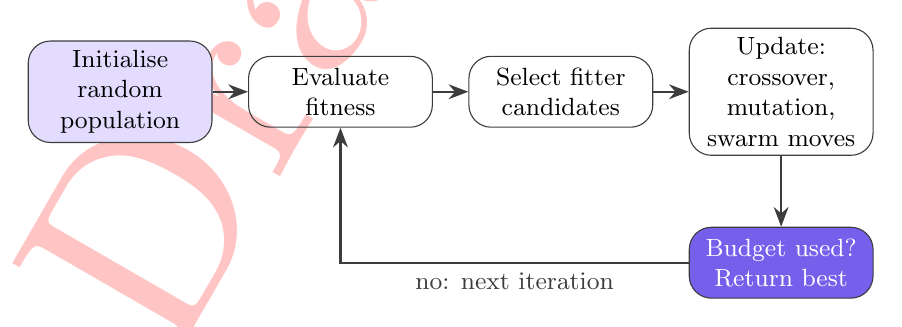
\begin{tikzpicture}[node distance=0.45cm, every node/.style={font=\small},
  box/.style={draw=ink, rounded corners=8pt, minimum height=0.9cm, text width=2.1cm, align=center},
  arr/.style={-{Stealth[length=2.5mm]}, thick, ink}]
\node[box, fill=lavender!40] (init) {Initialise random population};
\node[box, right=of init] (eval) {Evaluate fitness};
\node[box, right=of eval] (sel) {Select fitter candidates};
\node[box, right=of sel] (upd) {Update: crossover, mutation, swarm moves};
\node[box, fill=violet!80, text=white, below=0.9cm of upd] (stop) {Budget used? Return best};
\draw[arr] (init) -- (eval);
\draw[arr] (eval) -- (sel);
\draw[arr] (sel) -- (upd);
\draw[arr] (upd) -- (stop);
\draw[arr] (stop.west) -| node[pos=0.25, below] {no: next iteration} (eval.south);
\end{tikzpicture}
\caption{The general loop of a nature-inspired algorithm.}
\label{fig:loop}
\end{figure}

\section{Classification of Nature-Inspired Algorithms}
Table~\ref{tab:families} groups the algorithms into four families and marks those used in this project.

\begin{table}[H]
\centering
\caption{Families of nature-inspired algorithms.}
\label{tab:families}
\small
\begin{tabularx}{\textwidth}{|l|X|X|l|}
\hline
\textbf{Family} & \textbf{Inspired by} & \textbf{Examples} & \textbf{Used here} \\
\hline
Evolutionary & Natural selection and genetics & GA, Differential Evolution, Evolution Strategies & GA \\
\hline
Swarm intelligence & Collective behaviour of animals & PSO, GWO, WOA, HHO, CSO, Ant Colony & PSO, BPSO, GWO, \\
 & & & WOA, HHO, CSO \\
\hline
Physics/chemistry-based & Physical laws & Simulated Annealing, Gravitational Search & -- \\
\hline
Human/society-based & Human learning and social behaviour & Teaching--Learning-Based Optimisation, Harmony Search & -- \\
\hline
\end{tabularx}
\end{table}

\section{Genetic Algorithm}
The Genetic Algorithm \cite{holland1975} imitates natural selection. Each candidate is a chromosome; fitter
chromosomes are more likely to become parents; offspring are formed by crossover and mutation; and the population
evolves over generations.

\textbf{Encoding.} In this project a chromosome is a vector $x \in [0,1]^{1820}$, one gene per feature. It is decoded
into a feature subset by keeping the 50 features with the largest gene values (top-$k$ decoding), which always
satisfies the 50-feature constraint.

\textbf{Operators.} We use mealpy's BaseGA \cite{vanthieu2023} with its default operators:
\begin{itemize}
  \item \textbf{Selection:} tournament selection, with tournaments of 20\% of the population.
  \item \textbf{Crossover:} uniform crossover with probability $p_c = 0.95$; each gene is copied from either parent.
  \item \textbf{Mutation:} multi-point flip mutation with probability $p_m = 0.025$ per gene.
\end{itemize}

\begin{algorithm}[H]
\caption{Genetic Algorithm for feature selection}
\begin{algorithmic}[1]
\REQUIRE Standardised features, fitness $f$, budget of 1,000 evaluations
\ENSURE Best 50-feature subset
\STATE Initialise population $P$ of 20 random chromosomes in $[0,1]^{1820}$
\STATE Evaluate fitness $f(\mathrm{top}_{50}(x))$ for each $x \in P$
\FOR{generation $g = 1$ to $49$}
  \STATE Select parents by tournament selection
  \STATE Create offspring by uniform crossover ($p_c = 0.95$)
  \STATE Mutate offspring genes ($p_m = 0.025$)
  \STATE Evaluate offspring; keep the fittest as the next population
\ENDFOR
\RETURN the best 50-feature subset found
\end{algorithmic}
\end{algorithm}

\section{Particle Swarm Optimisation}
In PSO \cite{kennedy1995} each particle has a position $x_i$ and velocity $v_i$, and remembers its own best position
$p_i$ and the swarm's best position $g$:
\begin{equation}
v_i \leftarrow w\,v_i + c_1 r_1 (p_i - x_i) + c_2 r_2 (g - x_i), \qquad x_i \leftarrow x_i + v_i ,
\end{equation}
where $w$ is the inertia weight, $c_1, c_2$ are acceleration coefficients and $r_1, r_2$ are uniform random numbers.
\textbf{Binary PSO} keeps velocities continuous but sets each bit with a probability given by a transfer function:
the S-shaped sigmoid $1/(1 + e^{-v})$, or the V-shaped $|\tanh(v)|$, which flips a bit with that probability
\cite{mirjalili2013}.

\section{Grey Wolf Optimiser}
GWO \cite{mirjalili2014} models the leadership hierarchy and hunting of grey wolves. The three best solutions
($\alpha$, $\beta$, $\delta$) guide the others, and each wolf moves towards the average of positions suggested by
the three leaders. A coefficient $a$ decreases linearly from 2 to 0, so the search shifts from exploration to
exploitation over the iterations.

\section{Whale Optimisation Algorithm}
WOA \cite{mirjalili2016} imitates the bubble-net feeding of humpback whales. Each whale either encircles the best
solution, moves along a logarithmic spiral towards it, or (in exploration) moves towards a randomly chosen whale. As
in GWO, a decreasing coefficient controls the balance between exploration and exploitation.

\section{Harris Hawks Optimisation}
HHO \cite{heidari2019} models the cooperative hunting of Harris hawks. The prey's ``escape energy'' decreases over
time; when it is high the hawks explore, and when it is low they switch between soft and hard besieges, with rapid
dives that use L\'evy flights. HHO evaluates a variable number of candidates per iteration.

\section{Competitive Swarm Optimiser}
CSO \cite{cheng2015} was designed for large-scale optimisation. At each iteration the swarm is split randomly into
pairs, and the two particles of each pair compete. The winner passes to the next iteration unchanged; the loser
learns from the winner and from the swarm's mean position $\bar{x}$:
\begin{align}
v_{l} &\leftarrow r_1\, v_{l} + r_2\,(x_{w} - x_{l}) + \varphi\, r_3\,(\bar{x} - x_{l}), \\
x_{l} &\leftarrow \mathrm{clip}\!\left(x_{l} + v_{l},\; 0,\; 1\right),
\end{align}
where $r_1, r_2, r_3$ are random vectors in $[0,1]^D$ and $\varphi = 0.1$ controls the pull towards the mean.
Because only losers move, and they learn from many different winners, CSO keeps a diverse swarm and avoids the
premature convergence that standard PSO shows in high dimensions. With a swarm of 20, each iteration costs 10
evaluations.

\section{Why GA and CSO for Feature Selection}
GA was the strongest algorithm in our first study and is the most widely used method for feature selection. CSO was
chosen because it is built for problems with thousands of dimensions, like our 1,820-feature search space.
Table~\ref{tab:algos} summarises the algorithms studied.

\begin{table}[H]
\centering
\caption{Summary of the algorithms studied.}
\label{tab:algos}
\small
\begin{tabularx}{\textwidth}{|l|l|X|}
\hline
\textbf{Algorithm} & \textbf{Family} & \textbf{Key mechanism} \\
\hline
GA & Evolutionary & Selection, crossover and mutation over generations \\
\hline
PSO & Swarm & Particles pulled towards personal and global bests \\
\hline
Binary PSO (S, V) & Swarm & Velocity mapped to bit probabilities by a transfer function \\
\hline
GWO & Swarm & Leaders $\alpha$, $\beta$, $\delta$ guide the pack \\
\hline
WOA & Swarm & Encircling and spiral bubble-net moves \\
\hline
HHO & Swarm & Escape energy switches between exploration and besieges \\
\hline
CSO & Swarm & Pairwise competition; losers learn from winners and the mean \\
\hline
\end{tabularx}
\end{table}

% ============================================================ 5 METHODOLOGY
\chapter{Methodology and Implementation}

\section{System Architecture}
Figure~\ref{fig:pipeline} shows the pipeline of the main study. Each image is converted into 1,820 handcrafted
features; GA or CSO selects exactly 50 of them by maximising cross-validated accuracy on training images only; an
SVM is then trained on the selected features and evaluated once on the unseen test images.

\begin{figure}[H]
\centering
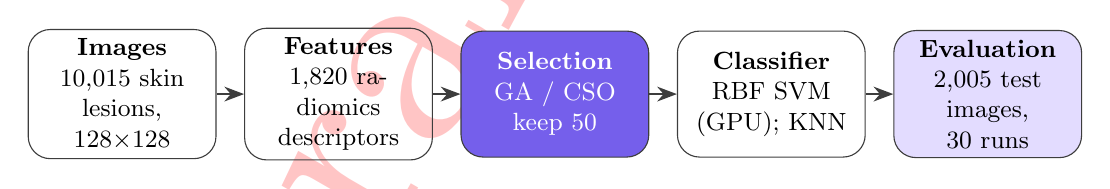
\begin{tikzpicture}[node distance=0.35cm, every node/.style={font=\small},
  box/.style={draw=ink, rounded corners=8pt, minimum height=1.6cm, text width=2.15cm, align=center},
  arr/.style={-{Stealth[length=2.5mm]}, thick, ink}]
\node[box] (img) {\textbf{Images}\\ 10,015 skin lesions, 128$\times$128};
\node[box, right=of img] (feat) {\textbf{Features}\\ 1,820 radiomics descriptors};
\node[box, right=of feat, fill=violet!80, text=white] (sel) {\textbf{Selection}\\ GA / CSO keep 50};
\node[box, right=of sel] (clf) {\textbf{Classifier}\\ RBF SVM (GPU); KNN};
\node[box, right=of clf, fill=lavender!40] (eval) {\textbf{Evaluation}\\ 2,005 test images, 30 runs};
\draw[arr] (img) -- (feat); \draw[arr] (feat) -- (sel); \draw[arr] (sel) -- (clf); \draw[arr] (clf) -- (eval);
\end{tikzpicture}
\caption{Pipeline of the main study on DermaMNIST.}
\label{fig:pipeline}
\end{figure}

\section{Datasets}
Four MedMNIST datasets were used (Table~\ref{tab:datasets}). The deep-feature studies used BreastMNIST and
RetinaMNIST; the handcrafted-feature studies used PneumoniaMNIST and DermaMNIST at 128\,$\times$\,128 pixels from
MedMNIST+, because texture features need more pixels than 28\,$\times$\,28 provides. All files matched the official
MD5 checksums.

\begin{table}[H]
\centering
\caption{Datasets used in the project.}
\label{tab:datasets}
\small
\begin{tabular}{|l|l|c|c|l|}
\hline
\textbf{Dataset} & \textbf{Modality} & \textbf{Train / Val / Test} & \textbf{Classes} & \textbf{Features used} \\
\hline
BreastMNIST & Breast ultrasound & 546 / 78 / 156 & 2 & ResNet-18 (deep) \\
\hline
RetinaMNIST & Retinal fundus & 1,080 / 120 / 400 & 5 & ResNet-18 (deep) \\
\hline
PneumoniaMNIST & Chest X-ray & 4,708 / 524 / 624 & 2 & Radiomics (1,359) \\
\hline
DermaMNIST & Dermatoscopy & 7,007 / 1,003 / 2,005 & 7 & Radiomics (1,820) \\
\hline
\end{tabular}
\end{table}

DermaMNIST, the main dataset, contains seven lesion types from HAM10000 \cite{tschandl2018}. It is strongly
imbalanced: melanocytic nevi make up 67\% of the training images (Table~\ref{tab:derma}).

\begin{table}[H]
\centering
\caption{DermaMNIST class distribution.}
\label{tab:derma}
\small
\begin{tabular}{|l|r|r|r|}
\hline
\textbf{Class} & \textbf{Train} & \textbf{Val} & \textbf{Test} \\
\hline
Actinic keratoses (AKIEC) & 228 & 33 & 66 \\
Basal cell carcinoma (BCC) & 359 & 52 & 103 \\
Benign keratosis (BKL) & 769 & 110 & 220 \\
Dermatofibroma (DF) & 80 & 12 & 23 \\
Melanoma (MEL) & 779 & 111 & 223 \\
Melanocytic nevi (NV) & 4,693 & 671 & 1,341 \\
Vascular lesions (VASC) & 99 & 14 & 29 \\
\hline
\textbf{Total} & \textbf{7,007} & \textbf{1,003} & \textbf{2,005} \\
\hline
\end{tabular}
\end{table}

\section{Baseline Reproduction and Deep Features}
For the deep-feature studies we used the released MedMNIST v2 ResNet-18 (28) weights, which reproduced the published
test scores exactly (BreastMNIST AUC 0.901, ACC 0.863; RetinaMNIST AUC 0.717, ACC 0.524). The 512-dimensional
global-average-pool output of each network was extracted for every image and used as the feature vector.

\section{Radiomics Feature Extraction}
For DermaMNIST, each 128\,$\times$\,128 colour image was converted into a fixed vector of 1,820 features using
scikit-image and SciPy (Table~\ref{tab:features}). No labels are used during extraction, so it cannot leak test
information. The greyscale features are computed on the luminance image; colour features use the RGB, HSV and
CIE~L*a*b* channels.

\begin{table}[H]
\centering
\caption{The 1,820 radiomics features extracted per image.}
\label{tab:features}
\small
\begin{tabularx}{\textwidth}{|l|r|X|}
\hline
\textbf{Group} & \textbf{Count} & \textbf{Content} \\
\hline
First-order and histogram & 52 & Intensity statistics (mean, spread, skewness, percentiles, entropy); 32-bin histogram \\
\hline
Spatial & 160 & Row and column band profiles; statistics in a 4\,$\times$\,4 grid \\
\hline
GLCM texture & 252 & 4 distances $\times$ 4 angles $\times$ 9 properties, plus per-quadrant averages \\
\hline
LBP & 214 & Uniform LBP at three radii, and per grid cell \\
\hline
HOG & 324 & 9 orientations, 32\,$\times$\,32-pixel cells \\
\hline
Filtered images & 300 & Haar wavelet sub-bands, Laplacian of Gaussian, Gabor filter bank \\
\hline
Edges and spectrum & 57 & Sobel and Canny edges; radial and angular FFT bands \\
\hline
Colour & 461 & Statistics and histograms of 9 colour channels; colour grid; centre-versus-surround contrast \\
\hline
\textbf{Total} & \textbf{1,820} & \\
\hline
\end{tabularx}
\end{table}

\section{Preprocessing}
All features are standardised (zero mean, unit variance) with a scaler fitted on the training and validation images
only. The scaler uses no labels and never sees the test set.

\section{Fitness Function}
\label{sec:fitness}
For a candidate $x$, the 50 features with the largest values of $x$ are selected, and the fitness is
\begin{equation}
f(x) = 1 - \mathrm{ACC}_{\mathrm{CV}}\big(\mathrm{top}_{50}(x)\big),
\end{equation}
the cross-validated error of the classifier on a fitness pool. For each run, the pool is a stratified random sample
of 3,000 of the 7,007 training images, split into 5 stratified folds. Because the number of features is fixed, no
size penalty is needed. Fitness values are cached, so a subset that is visited again is not re-evaluated.

\section{GPU Implementation}
One search makes 1,000 fitness evaluations, and each evaluation trains five classifiers (one per fold), so a single
run needs 5,000 classifier fits. To make this practical, the LS-SVM was implemented in PyTorch on the GPU. For a
feature subset, the kernel matrices of all five folds are built at once and the five linear systems (each with one
right-hand side per class) are solved in one batched call. Folds of unequal size are padded with identity rows that
do not change the solution. The implementation was validated against a NumPy float64 reference, and its float32
predictions agreed 100\% with float64. The KNN classifier was also implemented on the GPU and matched
scikit-learn's \texttt{KNeighborsClassifier} exactly.

\section{Implementation Details}
\begin{itemize}
  \item \textbf{Software and hardware:} Python 3.11, PyTorch 2.14 (CUDA 12.6), scikit-learn 1.9, scikit-image 0.26,
        SciPy 1.16, mealpy 3.0.3 \cite{vanthieu2023} and medmnist 3.0.2, on a laptop with an NVIDIA RTX 4060 GPU.
  \item \textbf{Algorithms:} mealpy BaseGA (population 20, 49 generations, default operators) and our own CSO
        \cite{cheng2015} (population 20, $\varphi = 0.1$); a hard cap stops every search at exactly 1,000
        evaluations, and all seeds are fixed for reproducibility.
\end{itemize}

% ============================================================ 6 EXPERIMENTAL SETUP
\chapter{Experimental Setup and Test Functions}

\section{Experimental Configuration}
Table~\ref{tab:config} lists the configuration of the main study.

\begin{table}[H]
\centering
\caption{Configuration of the main study (DermaMNIST).}
\label{tab:config}
\small
\begin{tabular}{|l|l|}
\hline
\textbf{Setting} & \textbf{Value} \\
\hline
Features & 1,820 radiomics features, standardised \\
Feature budget & exactly 50 features (2.7\%) \\
Fitness pool & 3,000 stratified training images, 5-fold CV \\
Evaluation budget & exactly 1,000 fitness evaluations per run \\
Population size & 20 \\
Runs & 30 per method, paired seeds (seed = run index) \\
Final model & trained on train + validation (8,010 images) \\
Test set & 2,005 images, scored once per run \\
Classifiers & RBF LS-SVM (main study), 5-NN (repeat study) \\
\hline
\end{tabular}
\end{table}

\section{Baseline Methods}
Every bio-inspired search was compared with three baselines that represent the pipeline \emph{without} a
nature-inspired algorithm:
\begin{itemize}
  \item \textbf{All features:} the classifier trained on all 1,820 features, with no selection.
  \item \textbf{Random search:} 1,000 random 50-feature subsets scored with the same fitness function, keeping the
        best. This is the key control: it shows whether gains come from the algorithm or simply from searching.
  \item \textbf{ANOVA filter:} the 50 features with the highest ANOVA F-scores on the run's fitness pool, a standard
        non-bio-inspired selection method.
\end{itemize}

\section{Test Functions and Benchmarks}
The ``test function'' optimised by every algorithm is the fitness function of Section~\ref{sec:fitness}: the
cross-validated error of the classifier for a 50-feature subset. Unlike standard benchmark functions such as Sphere
or Rastrigin, it is noisy, discrete and has no closed form, and each evaluation requires training classifiers. The
benchmark tasks are the four MedMNIST datasets, which differ in modality, size and number of classes.

Before running the main study we checked on training data only that the fitness function is meaningful. Over 60
random 50-feature subsets, the pool cross-validated accuracy ranked subsets in nearly the same order as accuracy on
the 4,007 training images outside the pool (Spearman $\rho = 0.83$). We also checked that the features are not
interchangeable: random 50-feature subsets scored 0.747 in cross-validation against 0.784 for all features, leaving
room for a search to find better subsets.

\section{Statistical Protocol}
The primary hypotheses, fixed before any test result was seen, were: GA vs random search, CSO vs random search, GA
vs filter and CSO vs filter, for test accuracy and test AUC. Each was tested with a two-sided paired Wilcoxon
signed-rank test over the 30 runs, with Holm correction over the four tests per metric. Macro-F1, balanced accuracy
and the comparison with all features were reported as secondary results.

\section{Repeat with a KNN Classifier}
To check that the result does not depend on one classifier, the whole study was repeated with a 5-nearest-neighbour
classifier in place of the SVM, in both the fitness function and the final model. Everything else (seeds, pools,
folds, budget and hypotheses) was identical.

\section{Deep-Feature Studies}
Before the radiomics study, six controlled studies tested feature selection on deep ResNet-18 features of
BreastMNIST and RetinaMNIST, with designs including validation-set fitness, cross-validated fitness, nested
cross-validation, fixed subset sizes and frozen ImageNet features. Together they comprised 1,470 search runs. Across
all four datasets the project performed 1,560 search runs.

% ============================================================ 7 RESULTS
\chapter{Results and Discussion}

\section{Main Results with the SVM}
Table~\ref{tab:d1} gives the test results of the main study, averaged over 30 runs, and Figure~\ref{fig:scores}
shows the result of every run.

\begin{table}[H]
\centering
\caption{DermaMNIST test results with the SVM, 50 features (mean $\pm$ standard deviation over 30 runs).}
\label{tab:d1}
\footnotesize
\begin{tabular}{|l|c|c|c|c|c|}
\hline
\textbf{Method} & \textbf{Features} & \textbf{Accuracy} & \textbf{AUC} & \textbf{Macro-F1} & \textbf{Bal.\ acc.} \\
\hline
All features (reference) & 1,820 & 0.803 & 0.954 & 0.541 & 0.480 \\
\hline
ANOVA filter & 50 & 0.765 $\pm$ 0.004 & 0.928 $\pm$ 0.004 & 0.496 & 0.442 \\
\hline
Random search & 50 & 0.770 $\pm$ 0.006 & 0.925 $\pm$ 0.007 & 0.458 & 0.410 \\
\hline
\textbf{GA} & 50 & \textbf{0.783 $\pm$ 0.006} & \textbf{0.936 $\pm$ 0.006} & 0.516 & 0.462 \\
\hline
\textbf{CSO} & 50 & \textbf{0.782 $\pm$ 0.006} & \textbf{0.935 $\pm$ 0.006} & \textbf{0.521} & \textbf{0.464} \\
\hline
\end{tabular}
\end{table}

\begin{figure}[H]
\centering
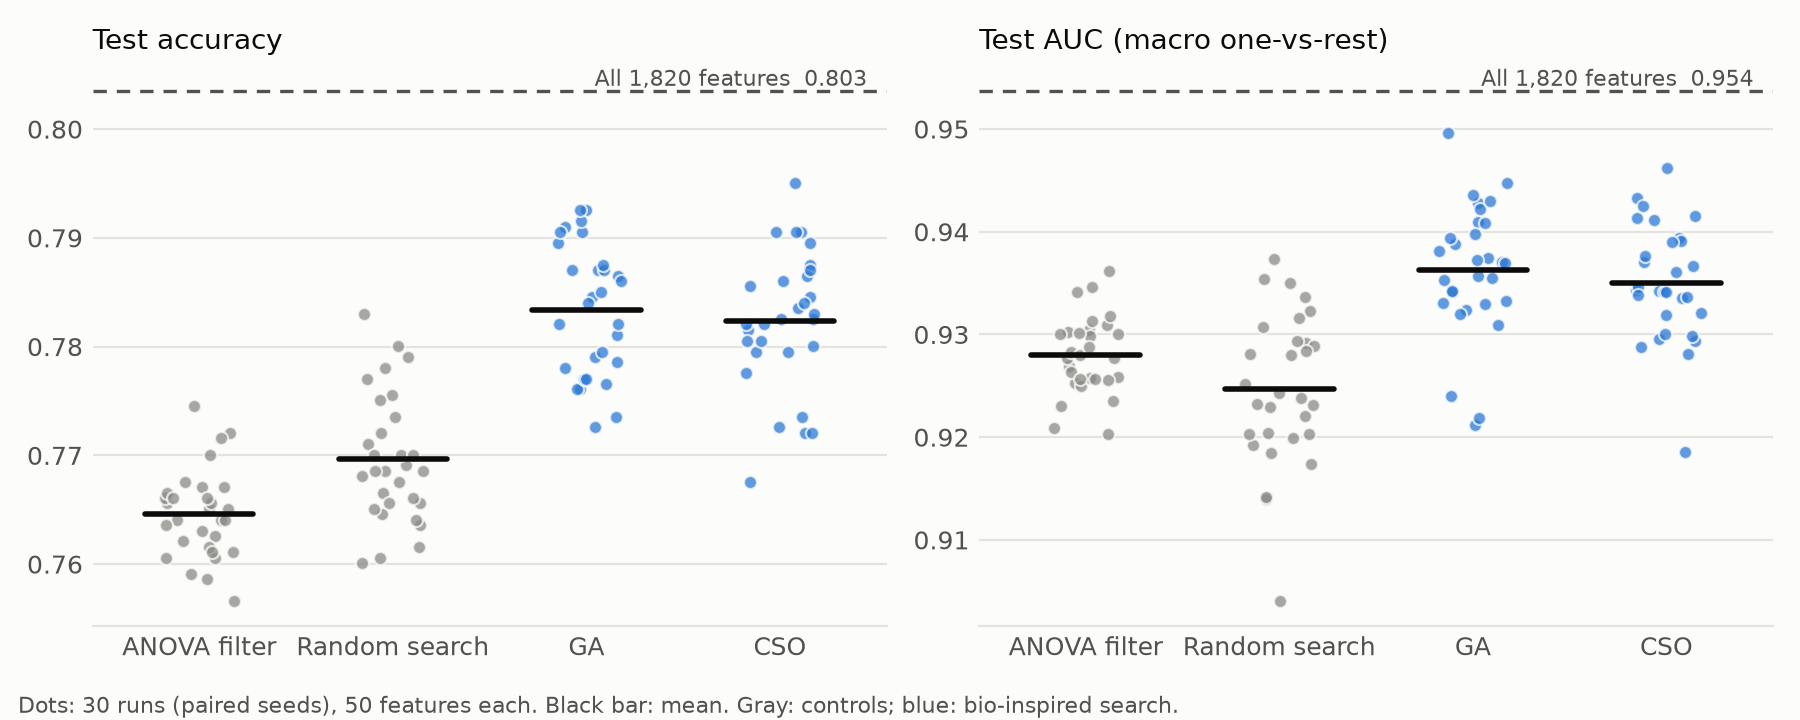
\includegraphics[width=\textwidth]{figures/test_scores.png}
\caption{Test accuracy and AUC of each of the 30 runs with 50 features. Black bars are means; the dashed line is the
model with all 1,820 features. Grey: baselines; blue: bio-inspired search.}
\label{fig:scores}
\end{figure}

GA reached a mean test accuracy of 78.3\%, against 77.0\% for random search and 76.5\% for the ANOVA filter, and a
mean test AUC of 0.936 against 0.925 and 0.928. CSO performed almost identically. GA had a higher accuracy than
random search in 27 of 30 runs and than the filter in all 30 runs.

\section{Statistical Significance}
All eight primary hypotheses were supported (Table~\ref{tab:d1tests}).

\begin{table}[H]
\centering
\caption{Primary hypothesis tests with the SVM (paired Wilcoxon, Holm-corrected over 4 tests per metric).}
\label{tab:d1tests}
\footnotesize
\begin{tabular}{|l|l|c|c|c|c|}
\hline
\textbf{Metric} & \textbf{Comparison} & \textbf{Mean diff.} & \textbf{Better/tied/worse} & \textbf{p} & \textbf{Holm p} \\
\hline
\multirow{4}{*}{Accuracy} & GA vs random search & +0.0138 & 27 / 0 / 3 & 5.0e-06 & 9.9e-06 \\
 & CSO vs random search & +0.0127 & 27 / 0 / 3 & 5.2e-06 & 9.9e-06 \\
 & GA vs filter & +0.0188 & 30 / 0 / 0 & 1.7e-06 & 6.9e-06 \\
 & CSO vs filter & +0.0177 & 29 / 1 / 0 & 1.8e-06 & 6.9e-06 \\
\hline
\multirow{4}{*}{AUC} & GA vs random search & +0.0116 & 26 / 0 / 4 & 2.0e-06 & 6.0e-06 \\
 & CSO vs random search & +0.0104 & 26 / 0 / 4 & 5.7e-07 & 2.3e-06 \\
 & GA vs filter & +0.0083 & 25 / 0 / 5 & 6.0e-06 & 6.0e-06 \\
 & CSO vs filter & +0.0071 & 27 / 0 / 3 & 2.8e-06 & 6.0e-06 \\
\hline
\end{tabular}
\end{table}

\section{Results with the KNN Classifier}
With the KNN classifier, all eight primary hypotheses were supported again (Table~\ref{tab:d2}). On accuracy, GA and
CSO beat random search by 1.3 to 1.5 percentage points and the filter by 1.7 to 1.9 points (Holm $p \le 2\times10^{-5}$).
On AUC they beat random search by 0.018 to 0.020 (Holm $p \le 6\times10^{-5}$); the AUC gains over the filter were
smaller (0.007 to 0.009, Holm $p = 0.031$--$0.035$). With KNN, GA's 50 features matched all 1,820 features on
accuracy (0.733 against 0.732), because KNN is easily confused by uninformative features.

\begin{table}[H]
\centering
\caption{DermaMNIST test results with the KNN classifier, 50 features (mean over 30 runs).}
\label{tab:d2}
\small
\begin{tabular}{|l|c|c|c|c|c|}
\hline
\textbf{Method} & \textbf{Features} & \textbf{Accuracy} & \textbf{AUC} & \textbf{Macro-F1} & \textbf{Bal.\ acc.} \\
\hline
All features (reference) & 1,820 & 0.732 & 0.834 & 0.420 & 0.426 \\
\hline
ANOVA filter & 50 & 0.714 & 0.806 & 0.420 & 0.401 \\
\hline
Random search & 50 & 0.718 & 0.795 & 0.393 & 0.384 \\
\hline
\textbf{GA} & 50 & \textbf{0.733} & 0.813 & \textbf{0.432} & 0.415 \\
\hline
\textbf{CSO} & 50 & 0.731 & \textbf{0.815} & 0.429 & 0.413 \\
\hline
\end{tabular}
\end{table}

\section{Results on Deep Features}
In contrast, on deep ResNet-18 features no bio-inspired algorithm significantly beat random search or all features
in any of the six deep-feature studies. The algorithms consistently raised their own fitness, but not the test
scores. Two reasons explain this:
\begin{itemize}
  \item \textbf{Redundancy.} Features from a network trained on the task are highly redundant: on BreastMNIST, a
        single random subset of 10 of the 512 features reached a test accuracy of 0.855 against 0.859 for all 512.
        When almost any subset carries the full signal, there is nothing for selection to find.
  \item \textbf{Over-fitting the fitness set.} On small datasets, a search of 1,000 evaluations over-fits the data
        used to score it (selection bias), so the gain on the fitness does not transfer to the test set.
\end{itemize}

\section{Discussion}
\subsection{Why Selection Works on Radiomics Features}
Radiomics features describe many distinct properties of an image, so a random 50 often misses the informative ones,
and a good search finds them. The fitness signal was also reliable ($\rho = 0.83$), so a better fitness carried over
to the test set. Both conditions were checked on training data before the study, and both failed on the deep
features.

\subsection{Advantages}
\begin{itemize}
  \item \textbf{Compact model:} 50 of 1,820 features (97\% fewer), with significantly higher accuracy than random or
        filter selection of the same size.
  \item \textbf{Robust across classifiers:} the gain appears with both SVM and KNN.
  \item \textbf{Gradient-free:} the search optimises any classifier's accuracy directly.
  \item \textbf{Parallel by design:} many candidate subsets can be scored at once on a GPU.
\end{itemize}

\subsection{Limitations}
\begin{itemize}
  \item \textbf{No gain on deep CNN features:} in 6 controlled studies (1,470 search runs), selection did not beat
        random search or all features.
  \item \textbf{Small accuracy cost:} with the SVM, the 50 selected features stay about 2 points below all 1,820
        features (0.783 against 0.803).
  \item \textbf{Compute-heavy:} every run trains 1,000 classifiers on five folds each.
  \item \textbf{Limited scope:} the positive result is from one dataset, with default algorithm settings.
\end{itemize}

% ============================================================ 8 COMPARATIVE ANALYSIS
\chapter{Comparative Performance Analysis}

\section{Bio-Inspired Search vs Baselines}
Table~\ref{tab:gains} summarises all 16 primary comparisons for both classifiers. Accuracy gains are in percentage
points (pp) with the relative gain in brackets; AUC gains are raw differences, also with the relative gain.

\begin{table}[H]
\centering
\caption{Gains of GA and CSO over the baselines on the test set (mean of 30 runs). All 16 are significant.}
\label{tab:gains}
\footnotesize
\setlength{\tabcolsep}{3.5pt}
\begin{tabular}{|l|c|c|c|c|}
\hline
\textbf{Comparison} & \textbf{SVM accuracy} & \textbf{SVM AUC} & \textbf{KNN accuracy} & \textbf{KNN AUC} \\
\hline
GA vs random search & +1.38 pp (+1.8\%) & +0.012 (+1.3\%) & +1.47 pp (+2.1\%) & +0.018 (+2.3\%) \\
\hline
GA vs filter & +1.88 pp (+2.5\%) & +0.008 (+0.9\%) & +1.85 pp (+2.6\%) & +0.007 (+0.9\%) \\
\hline
CSO vs random search & +1.27 pp (+1.7\%) & +0.010 (+1.1\%) & +1.33 pp (+1.9\%) & +0.020 (+2.5\%) \\
\hline
CSO vs filter & +1.77 pp (+2.3\%) & +0.007 (+0.8\%) & +1.71 pp (+2.4\%) & +0.009 (+1.1\%) \\
\hline
\end{tabular}
\end{table}

The gains have a similar size with both classifiers, which shows that they do not depend on one model. The largest
accuracy gains are against the ANOVA filter (about 1.8--1.9 pp); the largest AUC gains are against random search with
KNN (about 0.02).

\section{GA vs CSO}
GA and CSO did not differ significantly on any metric (accuracy $p = 0.48$, AUC $p = 0.56$ with the SVM). GA had a
slightly higher accuracy and AUC; CSO a slightly higher macro-F1 and balanced accuracy. Both are therefore suitable
for this task, and the choice between them can be made on convenience.

\section{Filter vs Random Search}
The two baselines have different strengths. With the SVM, the ANOVA filter had a slightly lower accuracy than random
search ($-0.5$ pp, $p = 0.002$) but a higher macro-F1 and balanced accuracy (+3 to 4 pp), because ANOVA ranking
favours features that separate the rarer classes. The bio-inspired searches beat both.

\section{SVM vs KNN}
Table~\ref{tab:svmknn} compares the two classifiers. The SVM is much more accurate in absolute terms, so it remains
the recommended model; the KNN study confirms that the bio-inspired gain is not specific to the SVM.

\begin{table}[H]
\centering
\caption{SVM and KNN compared for the GA-selected 50-feature model.}
\label{tab:svmknn}
\small
\begin{tabular}{|l|c|c|}
\hline
 & \textbf{SVM} & \textbf{KNN} \\
\hline
GA test accuracy & \textbf{0.783} & 0.733 \\
\hline
GA test AUC & \textbf{0.936} & 0.813 \\
\hline
Accuracy gain over random search & +1.38 pp & +1.47 pp \\
\hline
AUC gain over random search & +0.012 & +0.018 \\
\hline
AUC gain over filter (Holm p) & +0.008 ($6\times10^{-6}$) & +0.007 (0.035) \\
\hline
\end{tabular}
\end{table}

\section{Selected Features vs All Features}
With the SVM, both searches score lower than the 1,820-feature model in every run, by about 2.0 pp in accuracy and
0.018 in AUC, while using 2.7\% of the features. With KNN, GA's 50-feature model ties with all features on accuracy.
The value of bio-inspired selection here is therefore a compact model that is much better than other ways of
choosing a small subset, not an improvement over the full feature set.

\section{Deep Features vs Radiomics Features}
Table~\ref{tab:settings} contrasts the two settings and summarises why the outcome differed.

\begin{table}[H]
\centering
\caption{Why bio-inspired selection helped on radiomics features but not on deep features.}
\label{tab:settings}
\small
\begin{tabularx}{\textwidth}{|l|X|X|}
\hline
 & \textbf{Deep ResNet-18 features} & \textbf{Radiomics features (DermaMNIST)} \\
\hline
Feature redundancy & Very high: 10 random features $\approx$ all 512 & Low: random 50 lose about 4 CV points \\
\hline
Fitness reliability & Weak; over-fitted by the search & Strong ($\rho = 0.83$) \\
\hline
Fitness data & 78--1,200 images & 3,000-image pool per run \\
\hline
Result & No significant gain in 6 studies & Significant gain in all 16 comparisons \\
\hline
\end{tabularx}
\end{table}

% ============================================================ 9 APPLICATIONS
\chapter{Applications and Case Studies}

\section{Case Study: Skin-Lesion Classification}
The DermaMNIST study is itself a case study in computer-aided dermatology. Seven lesion types, including melanoma
and basal cell carcinoma, must be told apart from dermatoscopy images in which harmless nevi dominate. A 50-feature
model chosen by GA reaches 78.3\% accuracy and an AUC of 0.936, using a small set of texture and colour features that
can be computed quickly and inspected individually. For comparison, the MedMNIST v2 reference ResNet-18 (28) reports
0.735 accuracy and 0.917 AUC on this dataset at 28\,$\times$\,28 resolution; our models use 128\,$\times$\,128
images, so the numbers are not directly comparable.

\section{Computer-Aided Diagnosis in Low-Resource Settings}
Compact feature-based models need little memory and compute, and can run on ordinary laptops or mobile devices
without a GPU at inference time. This makes them suitable for screening tools in clinics with limited hardware,
where a deep network may be impractical.

\section{Interpretable Radiomics}
In radiology and oncology, radiomics models are valued because each feature has a clear meaning (for example, a
texture contrast or a colour statistic). Selecting 50 features instead of 1,820 makes it possible for clinicians to
review which properties the model relies on, an important step towards trustworthy clinical use.

\section{Other Applications of Bio-Inspired Feature Selection}
\begin{itemize}
  \item \textbf{Gene-expression analysis:} selecting a few informative genes from thousands for cancer
        classification, where small sample sizes make selection bias a central concern \cite{ambroise2002}.
  \item \textbf{Other medical imaging tasks:} chest X-ray, histopathology and MRI radiomics pipelines with large
        handcrafted feature sets.
  \item \textbf{Biosignals:} selecting features from ECG and EEG recordings for arrhythmia or seizure detection.
  \item \textbf{General machine learning:} any wrapper-based feature selection where the feature set is large and
        partly irrelevant.
\end{itemize}

\section{Lessons for Practitioners}
\begin{enumerate}
  \item Always compare with a random search of the same budget; without it, a gain may come from searching, not
        from the algorithm.
  \item Before a full study, check on training data that small random subsets lose accuracy and that the fitness
        ranks subsets reliably. If not, selection is unlikely to help.
  \item Use many paired runs and correct for multiple comparisons before claiming a significant improvement.
\end{enumerate}

% ============================================================ 10 CONCLUSION
\chapter{Conclusion}
This project tested, under strict and fair conditions, when nature-inspired feature selection improves medical image
classification. On deep ResNet-18 features of BreastMNIST and RetinaMNIST, eight algorithms gave no significant
improvement in six controlled studies, because the features were too redundant and the small fitness sets were
over-fitted.

On 1,820 handcrafted radiomics features of DermaMNIST, with a budget of 50 features, the Genetic Algorithm and the
Competitive Swarm Optimiser selected significantly better features than both random search and an ANOVA filter. With
an SVM, GA reached 78.3\% test accuracy and an AUC of 0.936, gains of 1.38 and 1.88 percentage points in accuracy
over random search and the filter. All 16 pre-specified comparisons, with both SVM and KNN classifiers, were
significant after Holm correction, and GA beat the filter in all 30 runs.

Bio-inspired feature selection is therefore not a general way to improve accuracy, but a valuable tool when the
features are not interchangeable and the fitness function is reliable. Both conditions can be checked on training
data before any test result is seen. In that setting it produces compact models, here 97\% smaller, that are
significantly better than other ways of choosing a small subset.

% ============================================================ 11 FUTURE WORK
\chapter{Future Work}

\section{Methodological Enhancements}
\begin{itemize}
  \item \textbf{Multi-objective selection:} use NSGA-II to trade accuracy against the number of features
        automatically, instead of fixing the budget at 50.
  \item \textbf{Hybrid filter and wrapper:} pre-filter to a few hundred features, then search, which is faster and
        may be more accurate.
  \item \textbf{Algorithm tuning:} tune population size, mutation rate and evaluation budget on a separate split.
\end{itemize}

\section{Richer Features and Data}
\begin{itemize}
  \item \textbf{Richer radiomics:} add the full pyradiomics set (GLRLM and GLSZM matrices) and use
        224\,$\times$\,224 images.
  \item \textbf{More datasets:} repeat the 50-feature study on other MedMNIST datasets and on clinical data.
\end{itemize}

\section{Clinical Validation}
\begin{itemize}
  \item \textbf{Interpretability:} ask dermatologists whether the selected texture and colour features make
        clinical sense.
  \item \textbf{Threshold tuning:} tune decision thresholds to raise recall on rare, dangerous classes such as
        melanoma.
\end{itemize}

% ============================================================ REFERENCES
\begin{thebibliography}{99}
\addcontentsline{toc}{chapter}{References}
\bibitem{yang2021} J.~Yang, R.~Shi and B.~Ni, ``MedMNIST classification decathlon: A lightweight AutoML benchmark for medical image analysis,'' in \emph{Proc. IEEE ISBI}, 2021.
\bibitem{yang2023} J.~Yang et al., ``MedMNIST v2 -- A large-scale lightweight benchmark for 2D and 3D biomedical image classification,'' \emph{Scientific Data}, vol.~10, p.~41, 2023.
\bibitem{doerrich2024} S.~Doerrich et al., ``Rethinking model prototyping through the MedMNIST+ dataset collection,'' arXiv:2404.15786, 2024.
\bibitem{aldhabyani2020} W.~Al-Dhabyani, M.~Gomaa, H.~Khaled and A.~Fahmy, ``Dataset of breast ultrasound images,'' \emph{Data in Brief}, vol.~28, p.~104863, 2020.
\bibitem{liu2022} R.~Liu et al., ``DeepDRiD: Diabetic retinopathy -- grading and image quality estimation challenge,'' \emph{Patterns}, vol.~3, p.~100512, 2022.
\bibitem{kermany2018} D.~S.~Kermany et al., ``Identifying medical diagnoses and treatable diseases by image-based deep learning,'' \emph{Cell}, vol.~172, pp.~1122--1131, 2018.
\bibitem{tschandl2018} P.~Tschandl, C.~Rosendahl and H.~Kittler, ``The HAM10000 dataset, a large collection of multi-source dermatoscopic images of common pigmented skin lesions,'' \emph{Scientific Data}, vol.~5, p.~180161, 2018.
\bibitem{haralick1973} R.~M.~Haralick, K.~Shanmugam and I.~Dinstein, ``Textural features for image classification,'' \emph{IEEE Trans. Systems, Man, and Cybernetics}, vol.~3, pp.~610--621, 1973.
\bibitem{ojala2002} T.~Ojala, M.~Pietik\"ainen and T.~M\"aenp\"a\"a, ``Multiresolution gray-scale and rotation invariant texture classification with local binary patterns,'' \emph{IEEE TPAMI}, vol.~24, pp.~971--987, 2002.
\bibitem{dalal2005} N.~Dalal and B.~Triggs, ``Histograms of oriented gradients for human detection,'' in \emph{Proc. CVPR}, 2005.
\bibitem{holland1975} J.~H.~Holland, \emph{Adaptation in Natural and Artificial Systems}. University of Michigan Press, 1975.
\bibitem{kennedy1995} J.~Kennedy and R.~Eberhart, ``Particle swarm optimization,'' in \emph{Proc. ICNN}, 1995.
\bibitem{mirjalili2013} S.~Mirjalili and A.~Lewis, ``S-shaped versus V-shaped transfer functions for binary particle swarm optimization,'' \emph{Swarm and Evolutionary Computation}, vol.~9, pp.~1--14, 2013.
\bibitem{mirjalili2014} S.~Mirjalili, S.~M.~Mirjalili and A.~Lewis, ``Grey wolf optimizer,'' \emph{Advances in Engineering Software}, vol.~69, pp.~46--61, 2014.
\bibitem{mirjalili2016} S.~Mirjalili and A.~Lewis, ``The whale optimization algorithm,'' \emph{Advances in Engineering Software}, vol.~95, pp.~51--67, 2016.
\bibitem{heidari2019} A.~A.~Heidari et al., ``Harris hawks optimization: Algorithm and applications,'' \emph{Future Generation Computer Systems}, vol.~97, pp.~849--872, 2019.
\bibitem{cheng2015} R.~Cheng and Y.~Jin, ``A competitive swarm optimizer for large scale optimization,'' \emph{IEEE Trans. Cybernetics}, vol.~45, pp.~191--204, 2015.
\bibitem{vanthieu2023} N.~Van Thieu and S.~Mirjalili, ``MEALPY: An open-source library for latest meta-heuristic algorithms in Python,'' \emph{Journal of Systems Architecture}, 2023.
\bibitem{suykens1999} J.~A.~K.~Suykens and J.~Vandewalle, ``Least squares support vector machine classifiers,'' \emph{Neural Processing Letters}, vol.~9, pp.~293--300, 1999.
\bibitem{ambroise2002} C.~Ambroise and G.~J.~McLachlan, ``Selection bias in gene extraction on the basis of microarray gene-expression data,'' \emph{PNAS}, vol.~99, pp.~6562--6566, 2002.
\bibitem{cawley2010} G.~C.~Cawley and N.~L.~C.~Talbot, ``On over-fitting in model selection and subsequent selection bias in performance evaluation,'' \emph{JMLR}, vol.~11, pp.~2079--2107, 2010.
\bibitem{wilcoxon1945} F.~Wilcoxon, ``Individual comparisons by ranking methods,'' \emph{Biometrics Bulletin}, vol.~1, pp.~80--83, 1945.
\bibitem{holm1979} S.~Holm, ``A simple sequentially rejective multiple test procedure,'' \emph{Scandinavian Journal of Statistics}, vol.~6, pp.~65--70, 1979.
\end{thebibliography}

% ============================================================ GITHUB
\chapter*{\centering GitHub Repository Link}
\addcontentsline{toc}{chapter}{GitHub Repository Link}
The complete source code, including feature extraction, the GPU fitness function, the algorithm implementations,
the experiment runners and the analysis scripts, is available at:

\begin{center}
\url{https://github.com/a1l2v/bio-inspired-feature-selection}
\end{center}

\end{document}
